\documentclass[10pt, conference, compsocconf]{IEEEtran}
\hyphenation{op-tical net-works semi-conduc-tor}

\usepackage{cite}
\usepackage{epsfig}
\usepackage{graphicx}
\usepackage{subfigure}

\begin{document}
\bibliographystyle{IEEEtran}

\title{Online Training Machine Learning based Runtime Decision Maker for
Mobile Offloading Framework}

\author{\IEEEauthorblockN{Heungsik Eom, Renato Figueiredo}
\IEEEauthorblockA{Advanced Computing and Information Systems Laboratory\\
Electrical and Computer Engineering\\
University of Florida, Gainesville, Florida, USA\\
\{hseom, renato\}@acis.ufl.edu}
\and
\IEEEauthorblockN{Huaqian Cai, Gang Huang}
\IEEEauthorblockA{Operating System and Middleware Laboratory\\
School of Electronics Engineering and Computer Science\\
Peking University, Beijing, China\\
\{caihq12, hg\}@pku.edu.cn}
}

\maketitle

\begin{abstract}
%
OpenCL has emerged as the open standard for parallel programming for
heterogeneous platforms enabling a uniform framework to discover,
program, and distribute parallel workloads to the diverse set of compute
units in the hardware.
%
For that reason, there have been efforts exploring the advantages of
parallelism from the OpenCL framework by offloading GPGPU workloads
within an HPC cluster environment.
%
In this paper, we present an OpenCL-based remote offloading framework
designed for mobile platforms by shifting the motivation and
advantages of using the OpenCL framework for the HPC cluster environment
into mobile cloud computing where OpenCL workloads can be exported from
a mobile node to the cloud.
%
Furthermore, our offloading framework handles service discovery, access
control, and data privacy by building the framework on top of a social
peer-to-peer virtual private network, SocialVPN. 
%
We developed a prototype implementation and deployed it into local- and
wide-area environments to evaluate the performance improvement and
energy implications of the proposed offloading framework.
%
Our results show that, depending on the complexity of the workload and
the amount of data transfer, the proposed architecture can achieve more
energy efficient performance by offloading than executing locally.
\end{abstract}

\begin{IEEEkeywords}
Mobile device, OpenCL, heterogeneity, parallelism, virtual private
networks, energy consumption
\end{IEEEkeywords}

\section{Introduction}
%
Over the last decade, remote offloading techniques have emerged as
intelligent means to overcome the constraints of the limited resouces
from mobile platforms, smartphones and tabletPCs, so that these types of
devices delegate computationally intensive computing tasks to more
powerful external resources such as personal workstations or cloud
servers.
%
Initially, most of research interests on remote offloading techniques
have focused on core mechanisms in which \textit{what to offload} and
\textit{how to offload} have been primarily considered. 
%
The reseach community has studied various approaches to offload mobile
computations such as application partitioning~\cite{spectra, maui,
cuckoo}, thread migration~\cite{clonecloud, comet}, and application
migration~\cite{hung}.\\
%
\indent However, benefits from offloading computation-intensive portions
of mobile applications can be influenced by various internal and
external factors such as application requirements, network condition,
and computing capabilities of mobile or external devices.
%
Thus, \textit{whether to offload or execute locally} needs to be
decided constantly by considering and monitoring abovementioned fynamic
features on runtime.
%
Otherwise, incorrect offloading decision may cause the performance
degradation or worse energy consumption.
%
For that reason, research focuses have been naturally shifted into
dynamic scheduling or decision making problems for mobile offloading
framework.
%
For example, Kwon et al.~\cite{kwon} consider a simple rule-based
decision maker in which the framework decides to offload the mobile
computation only when the data transfer size is greater than the certain
threashold.
%
MAUI~\cite{maui} utilizes a linear regression model among predefined
features to make offloading decision.
%
%Also our previous paper suggested to apply machine learning
%techniques to the adaptive scheduling problem for mobile offloading
%framework by considering various machine learning algorithms~\cite{ml}.
%
Even though these studies on making offloading decision take dynamic
features such as data transfer size or network conditions into account
to make offloading decisions, it is impractical to generalize these
efforts for various mobile use case scenario, since they utilized
application-dependent decision making models.
%
Therefore, in practice, it is essential for decision maker to learn
from self-observation of the previous decision correctness and to
dynamically adapt the decision policy on runtime so that it can be
\textit{generally} applied to various mobile applications.\\
%
\indent In this paper, we aim to build an online framework to train 

%
\indent The rest of the paper is organized  as follows.
%
In Section II, we overview previous studies on offloading decision
problems in mobile offloading frameworks, as well as the use of machine
learning techniques for various scheduling problems.
%
Section III discusses the challenges in online training machine learing
runtime scheduler for mobile offloading framework.
%
In Section IV and V, we explain and evalute our implementation of the
online training ML scheduler.
%
Also, Section VI describes the current and potential applications for
our work.
%
Finally, we conclude the paper in Section VII.
%
\section{Motivation}
%
In this section, we describe a scenario that motivates our approach.
%
Figure 1 gives a general idea of one example deployment scenario.
%
Alice connects her smartphone to a virtual private network (VPN) consisting 
of her laptop, Bob's desktop, and her virtual machine running on Amazon EC2.
%
Since each of these devices is running SocialVPN~\cite{socialvpn}, they 
automatically join the same virtual private network creating a pool of trusted 
resources in a Social Device Network.
%
With this secure IP layer consisting of trusted peers, our framework is 
able to use IP multicasting over the VPN to discover nodes that are available 
for computation offloading.
%
During the discovery process, our system records the characteristics of each 
node in the network such as bandwidth, latency, and processing capabilities.
%
When an application decides to offload some computation, our framework 
dynamically determines the best node to use as the remote offloading target.
%
In many cases, for example, if the bandwidth or remote processing capabilities 
are not adequate, our framework may decide to simply run the workload
locally.\\
%
\indent By linking to our library, the developer can transparently access remote 
resources available via the SocialVPN, including GPUs running on computing
resources which is more powerful than a mobile 
device.
%
For example, if the mobile device is connected to a virtual network 
consisting of an Amazon EC2 GPU instance, and the workstation of the
mobile user, our extensions to the OpenCL framework will automatically 
select the best candidate based on available device capabilities and 
network conditions as the target compute node for remote execution.
%
Also, the use of SocialVPN ensures that the computation is offloaded securely
to socially trusted nodes.
%
This enhancement occurs transparently to the developer and the user 
requiring only code recompilation.
%
We perform various experiments in our analysis to demonstrate the 
feasibility of this integration.\\
%
\indent The goal of our design is to provide an intuitive offloading framework that 
developers can integrate into their application using well-adopted 
programming concepts.
%
We aim to extend the umbrella of heterogeneous computing to include devices
beyond the physical host platform.
%
Currently, many software developers utilize the OpenCL framework to exploit 
on-board heterogeneous platforms.
%
Popular software projects, such as OpenCV and OpenSSL, are re-implementing
major portions of their functions to run on the OpenCL
platform~\cite{opencv}.
%
Mobile SoC platforms, based on processors such as ARM and Intel, are also 
starting to provide OpenCL support on their architecture.
%
The latest version of the OpenCL specification allows for devices beyond 
CPUs and GPUs to be accessed through the API. 
%
There is also an industry momentum building up behind OpenCL with the
formation of new industry foundations to foster fast adoption~\cite{hsa}. 
%
These considerations point to OpenCL API as the emerging de facto standard 
for heterogeneous computing.
%
\begin{figure}
\centering
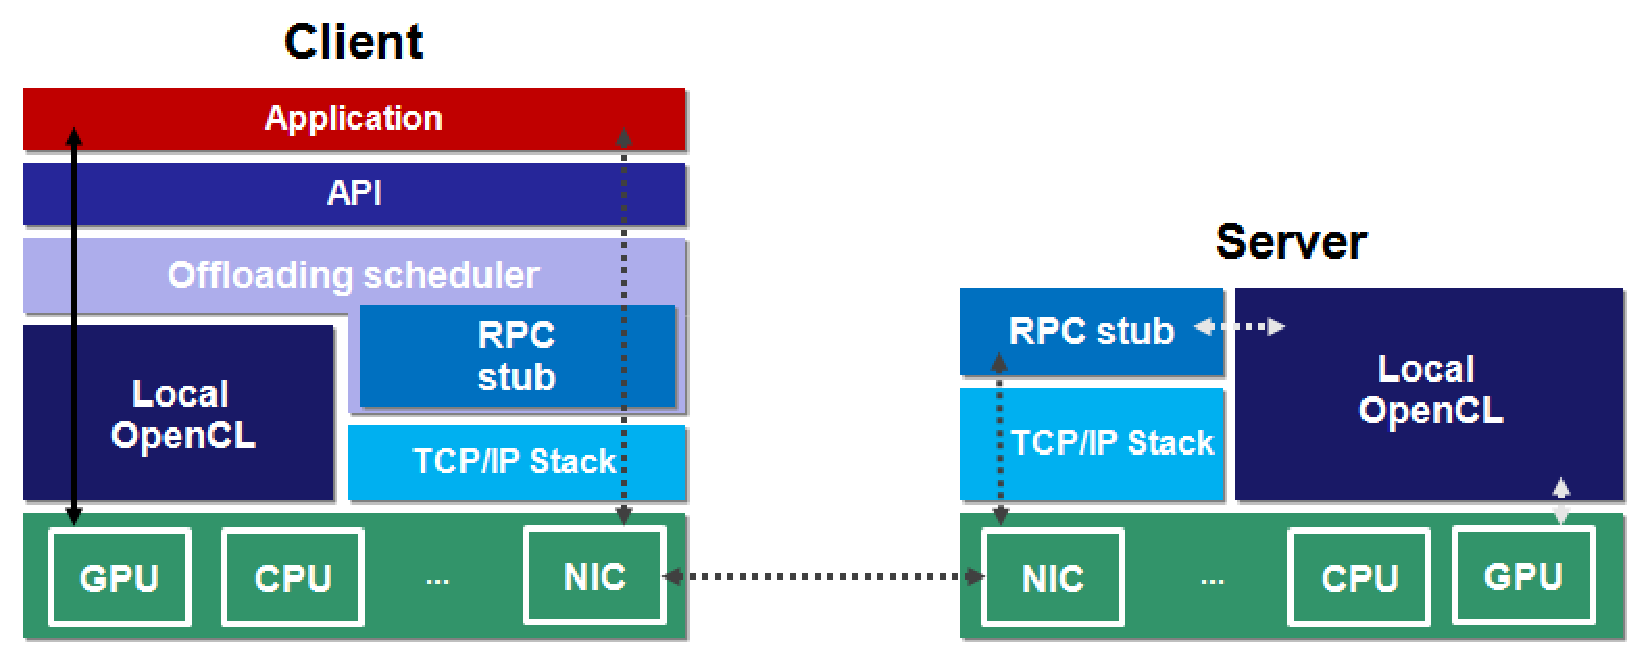
\includegraphics[height=3.4cm, width=8.5cm]{Figure/architecture}
\caption{The overall system architecture.}
\end{figure}
%
\section{Offloading Framework}
%
Our overall architecture consists of five main modules: integration with the 
OpenCL API, RPC-based offloading mechanism, runtime scheduler, decentralized resource discovery 
feature, and trusted, private IP communication layer.
%
The overall system architecture is shown in Figure 2.
%
\subsection{Transparent OpenCL API Integration}
%
Since OpenCL is an open standard currently supported by most of the major 
device manufacturers, we chose not to deviate from their API in order to 
minimize the learning curve for developers. 
%
Latest revisions of the OpenCL specification are extending the coverage to 
enable integration of a large pool of heterogeneous hardwares under the API.
%
Because OpenCL is also a hardware level offloading framework, it provides 
various functions that we can leverage in our system.
%
The OpenCL API possesses these set of features: device discovery and 
enumeration, device selection and customization, buffer management, job 
offload and status queries.
%
With these features, the application developer has full control on the 
use of specific accelerators necessary to optimize their application 
performance.
%
Here we explain how we extend each functionality to support remote
offloading.\\
%
\indent\textbf{Discovery and Enumeration.}
In the initialization phase of the interface, the developer queries the 
platform for on-board OpenCL-capable accelerators.
%
The OpenCL framework returns a list of accessible compute devices located 
on-board the device along with their capabilities (e.g. graphics cards, video 
decoders, cryptographic devices).
%
We extend this portion of the API by allowing the developer to discover other 
OpenCL-enabled accelerators located on remote nodes over the network. 
%
Hence, when the developer performs this query on a mobile device, it may 
discover not just the mobile GPU but also another GPU running on the cloud,
as long as they are part of the same virtual private network.\\
%
\indent\textbf{Selection and Configuration.}
In the standard OpenCL framework, once presented with a list of devices, the 
developer selects one or more targets for computation offloading.
%
This selection is usually based on the characteristics of each particular 
device, (e.g. number of compute units of the accelerator, maximum number of 
work items, architecture, latency and so on).
%
By extending the discovery process to include remote OpenCL devices over 
the network, this selection and configuration process can become cumbersome 
to the developer.
%
Thus, our system can present just one virtual device handle which represents
the best offloading node according to network conditions.
%
Our analysis shows that bandwidth and latency have the most impact on the 
performance.\\
%
\indent\textbf{Workload State Transfer.}
Having selected a device, the next phase is the actual offloading of the data
and code necessary to run remotely.
%
The function to be executed (called a kernel) is first sent either as C99 
source code or an LLVM-based intermediate language.
%
Once transferred, the code is compiled for the target accelerator.
%
In order to execute the kernel on the accelerator, the necessary state 
has to be transferred to the device regardless of whether it is local or 
remote.
%
If the device resides on the host platform, the task of buffer management 
simply involves copying data from main memory to local storage accessible 
by the accelerator.
%
However if the workload is being offloaded to a remote accelerator, then 
the buffers have to be managed slightly differently.
%
First, the data has to be marshalled and copied into the networking stack’s
buffers then transported over the network to the appropriate remote host.
%
The data is then copied from the remote host’s networking stack unto the 
accelerator’s own local storage.
%
Upon completion, the output buffers are copied back from the GPU’s local 
memory to the mobile device’s memory over the network.\\
%
\indent\textbf{Resource and Failure Management.}
The final phase of the OpenCL API is the ability to discover errors and 
release its state and resources in a graceful manner.
%
Each function has its error parameter which keeps the developer aware of 
the proper execution of the remote job.
%
If an error occurs due to an issue with the source code, or the workload 
configuration, or any other hardware issues, an appropriate error code is 
returned to the developer.
%
In return, the developer can release the various resources (e.g. buffers, 
device handles) that are associated with the job.
%
Once again, we extend this functionality to support network failures as well.
%
In case of a disconnection, the appropriate error code is returned to the 
developer who then performs the necessary actions to clean up the state 
belonging to the job.
%
On the server, the necessary clean-up is taken as well by our framework.
%
Our decision to utilize the OpenCL framework for computation offloading in 
mobile devices allows us to leverage all of the functionalities already in 
place for offloading computation locally from the CPU to an on-board hardware 
accelerator.
%
\subsection{RPC-based Computation Offloading}
%
In order to support offloading on the remote node, we create an RPC-based 
service which handles offloading requests received over the virtual private 
network.
%
In our first attempt, we utilized SunRPC to provide the remote procedure 
calling interface, serialization, and networking capabilities.
%
However, SunRPC provides many extra features that were not necessarily 
efficient (for example, the use of a portmapper daemon to discover the 
listening port of the RPC service).
%
SunRPC also initiates a new TCP connection for each function call which 
incurs extra delay and poorer network performance.
%
In contrast, our design uses a single TCP connection per offloading job thus
achieving lower latencies.
%
By running an RPC service which exposes the OpenCL API over the network, we 
provide a computation offloading design that is lightweight in terms of 
argument serialization and buffer management.
%
Other approaches~\cite{vocl} rely on more sophisticated communication primitives such
as MPI which require extra processing and memory resulting in poor battery 
performance.
%
\begin{figure*}[ht]
%\begin{figure}
\centering
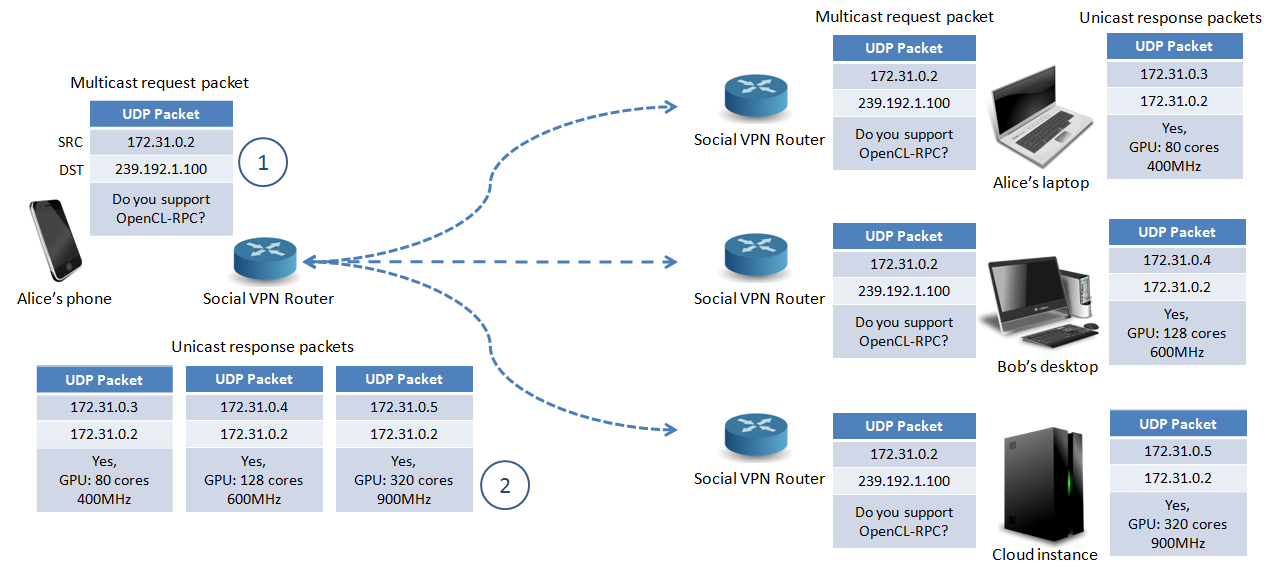
\includegraphics[height=6.3cm, width=13.8cm]{Figure/discovery}
\caption{Decentralized multicast service discovery.
%
1) The mobile device sends on IP multicast packet to the SocialVPN
software router running on the local device.
%
The SocialVPN router forwards the multicast packet to each device in
private network who are running the SocialVPN software router locally.
%
2) Each remote endpoint sends back a unicast UDP packet to the mobile
device.
%
Each response also contains the accelerator's computing capabilities.
%
Our system records the latency and computing capabilities which allow
the scheduler to determine the best offloading node.
}
\end{figure*}
%
\subsection{Runtime Scheduling}
%
As previously mentioned, our enhanced OpenCL framework provides developers 
with a list of accelerators (both local and remote) to select as offload 
targets.
%
However, some applications developers may not want to bother with the task
of figuring out which devices would make a good candidate for local versus 
remote offloading.
%
Our framework includes a simple scheduler that can use latency to determine
dynamically if a workload should be offloaded or run locally.
%
The default behavior is to offload the computation to the node with the 
lowest latency.
%
This is an overly simplistic model which can be extended to consider 
various different properties.
%
In the future, we plan on supporting a more complex set of conditions along
with heuristics which optimizes for better battery performance.
%
The scope of this paper is to differentiate which scenario is ideal for our
offloading framework; our analysis provides a base to develop a more 
sophisticated scheduler moving forward. 
%
\subsection{Decentralized Resource Discovery}
%
Current mobile offloading solutions rely on a centralized service to provide
this resource discovery capability.
%
A key differentiation of our approach is our decentralized IP multicast-based
service discovery subsystem.
%
Because we deploy our system on top of SocialVPN which enables IP-multicasting
over the Internet, we are able to leverage existing LAN-based service discovery 
techniques.
%
The discovery process works in the following manner: the client periodically
polls the network for eligible offloading nodes by sending a UDP datagram to
the multicast IP address.
%
The SocialVPN router distributes the IP packet to every node in the private 
network.
%
The RPC-based service described earlier has a UDP listening thread that waits
for service discovery request and responds to the request with its computing
capabilities using the request’s unicast IP address.
%
The requester waits for a certain amount of time and accumulates all the 
replies that it receives within that time window.
%
The requestor records their latency, bandwidth, and processing capabilities
and provides that to the scheduler.
%
The scheduler then determines which node will provide the best performance
and selects that node as the offloading candidate.
%
Figure 3 depicts the decentralized multicast service discovery.
%
\subsection{Trusted Communication via VPN}
%
The virtual networking component addresses two key challenges of remote 
workload offloading -- privacy and peer discovery -- while supporting 
unmodified TCP/IP applications to offload computation to remote accelerators.
%
In order to augment computing capabilities of the mobile platforms, it is 
important to find trusted nodes that are not just in the same local area
network, but also geographically-dispersed peers, and to do so dynamically and 
transparently to the mobile application.
%
SocialVPN ensures that peers anywhere on the Internet appear to be on the
same virtual LAN and end-to-end encrypted peer-to-peer tunnels are abstracted
as virtual IP links among peers.
%
By leveraging SocialVPN as a trusted peer-to-peer messaging substrate, we
are able to use the Berkeley sockets networking interface to offload our
workload without any direct linking to SocialVPN itself.
%
Most peer-to-peer systems require integration with a P2P library as well as a 
learning curve for learning its API.
%
Because SocialVPN provides virtual private IP addresses to peers instead of
P2P addresses, it supports unmodified applications.
%
\section{Evaluation}
%
In this section, we evaluate the implementation of the OpenCL-based remote
offloading framework for mobile platforms in terms of the performance 
improvement and energy consumption for mobile devices through real deployment
over local- and wide-area environments.
%
We first examine the overhead of adopting SocialVPN to the secure 
communication between the client and the server since SocialVPN utilizes 
its own encryption and IP tunneling.
%
Then, we characterize the benefits and costs of our remote offloading 
framework through a series of experiments using various OpenCL 
workloads.
%
\subsection{Experimental Setup}
%
In order to evaluate our remote offloading framework under a variety of 
possible use case scenarios, we setup the experiment using various hardware
and network configurations.
%
First of all, our hardware setup consists of a client and three server types.
%
For the mobile client, we utilized an Android tablet, Samsung GalaxyTab 10.1 
equipped with 1GHz dual-core processor and 1GB RAM, and running Android 3.1.
%
One of the servers is a workstation with an Intel 3.0 GHz Core2 Duo
processor running Ubuntu 12.04 with 8GB RAM.
%
Second server has same features as first server, but it is equipped with
an Nvidia Geforce GT 640 GPU with 2GB RAM.
%
Last configuration for the server is an Amazon EC2 GPU instance with 16 vCPUs, 22.5GB RAM,
and two Nvidia Tesla GPUs running Ubuntu 12.04.
%
We ran our experiments on the different networks: 1) a LAN within the lab
with an average bandwidth of 6.5MB and 10ms latency, 2) the campus
wireless network with an average bandwidth of 2.5MB and 15ms latency,
3) the Internet connection to Amazon EC2 with an average bandwidth of
0.17MB and 74ms latency.\\
%
\indent We utilized OpenCL SDK code samples provided by AMD APP SDK~\cite{amd} and 
Nvidia~\cite{nvidia} as the offloaded workloads to measure the efficacy and the cost
of our remote offloading framework.
%
We selected four workloads each with different characteristics.
%
\textit{Sobelfilter} is an image processing workload for edge detection, we
classify it as a high state transfer and low computation workload.
%
The second workload is an \textit{Hidden-Markov} model workload, a popular
statistical tools for modeling sequences as well as machine learning;
this represents a low state transfer and high computation workload.
%
We also tested a \textit{matrix multiplication} as one of the workloads because
it is a common operation for scientific computing.
%
Finally, an \textit{N-body Physics} workload which is a common
mathematical simulation method for modeling astronomical objects;
this is considered a high state transfer and high computation workload.
%
These workloads provide some insight into which use cases best fit our
mobile cloud offloading scenario through our OpenCL-based offloading framework.
%
\begin{figure}
\centering
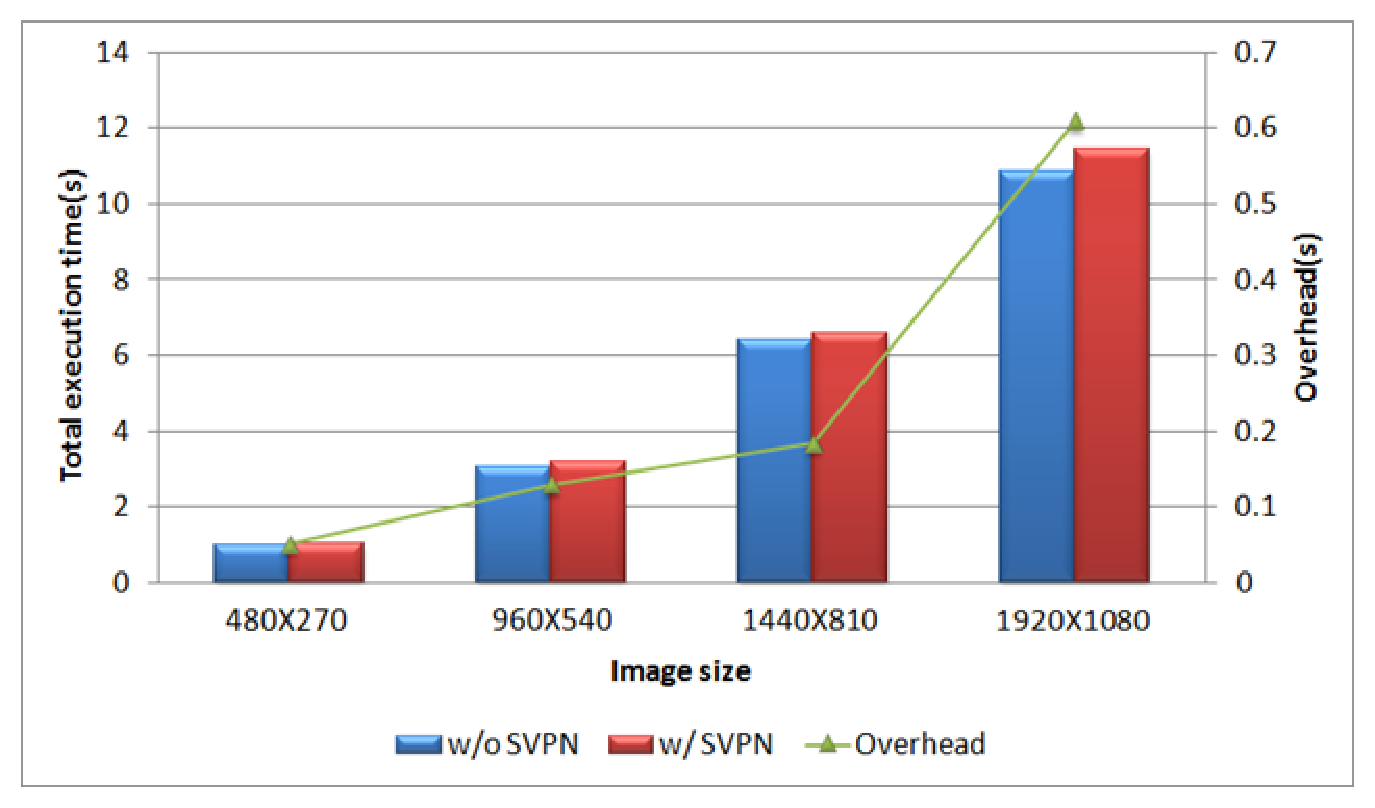
\includegraphics[height=4.5cm, width=7.5cm]{Figure/svpn1}
\caption{Execution time with and without SocialVPN.
}
\end{figure}
%
\begin{figure}
\centering
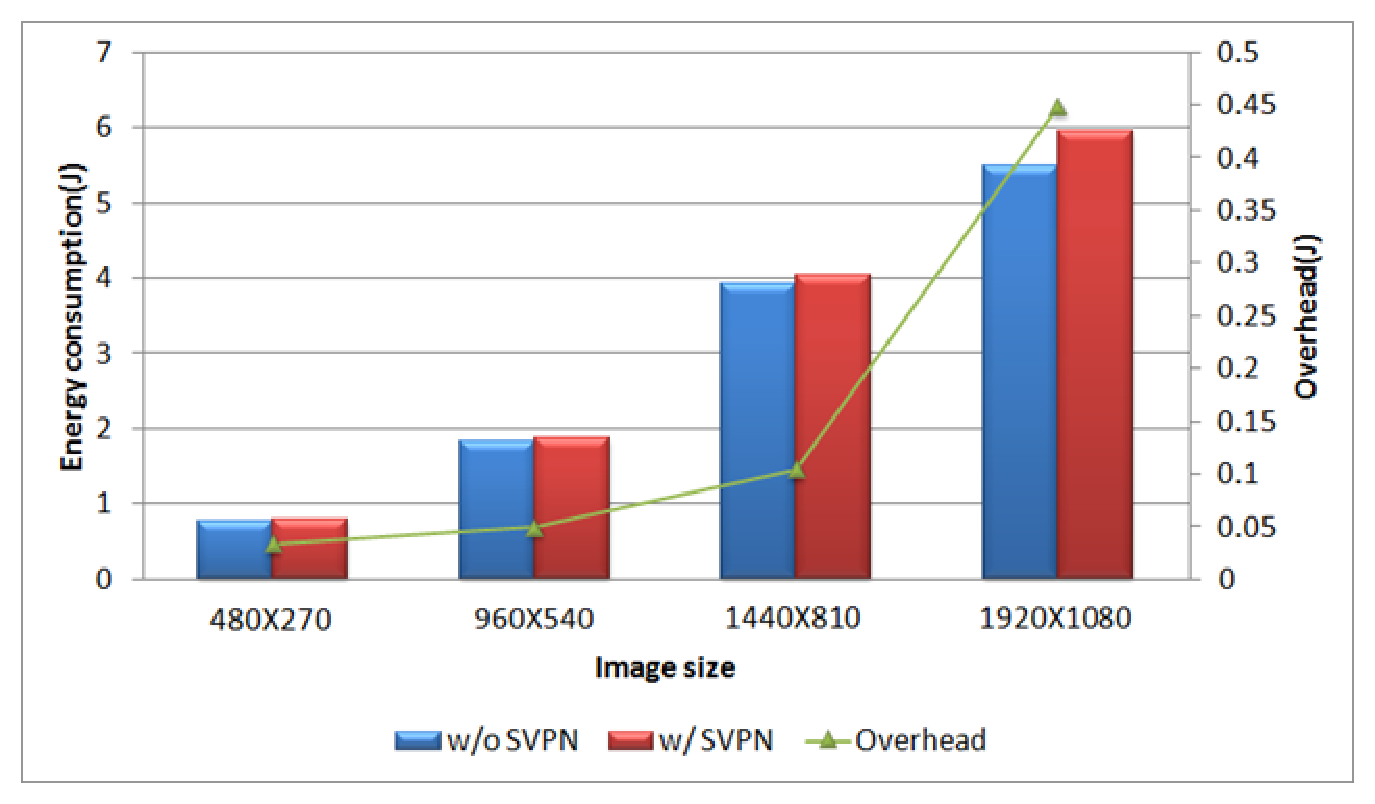
\includegraphics[height=4.5cm, width=7.5cm]{Figure/svpn2}
\caption{Energy consumption with and without SocialVPN.
}
\end{figure}
%
\subsection{Overhead of SocialVPN}
%
In our remote offloading framework, SocialVPN enables mobile devices and 
remote resources to securely communicate which incurs some overhead due to 
encryption and tunneling.
%
In this section, we investigate the overhead of SocialVPN with respect to
the performance and energy consumption.
%
In order to measure the overhead of SocalVPN, we have conducted the 
LAN experiments in which the client offloads an OpenCL
workload (Sobelfilter) to the server
both with and without SocialVPN.
%
As shown in Figure 4 and 5, as the image size increases, the execution time 
and energy consumption also increase.
%
In the case of 480$\times$270 of image, for instance, offloading with SocialVPN
takes 0.05 seconds more than without SocialVPN while it takes 0.6s more to
offload 1920$\times$1080 image which means that the overhead ranges from 2.8\% 
to 5.6\%.
%
In Figure 5, we also observed the overhead ranging from 2.6\% to 8.1\% in
terms of energy consumption.
%
\subsection{Performance and Energy Consumption Analysis}
%
As mentioned above, we have utilized three types of servers for the 
different server’s computing capabilities: CPU only-installed server, 
GPU-installed server and Amazon EC2 GPU cluster instance.
%
For various network configurations, we used a local area network in which
the client and the server directly connect via a wireless router, and a wide 
area network using campus network and traffic shaping.
%
For Sobelfilter and matrix multiplication, we varied the image and matrix 
sizes to measure the impact of the amount of data transfer and computation.
%
Also, Sobelfilter and matrix multiplication require 7 and 8 of one-time 
argument setups through the API called \textit{clSetKernelArgs} which causes additional
overhead to setup the extra arguments for kernel executions, respectively.
%
For hidden Markov model, the different number of states is used to vary 
the size of input; however, the kernel execution is repeated 100 times each 
requiring 10 of argument setup calls (i.e. total 1000 of argument 
setup calls) which make the hidden Markov model workload most 
communication-intensive.
%
In contrast with other workloads, however, N-body physics varies the 
number of the iterations that the kernel is executed on the server with
a same data set processed for each iteration.
%
Thus, regardless of the number of iterations, the size of input and output
data is identical, but as the number of iterations increases, the number of
argument setup calls proportionally increases.\\
%
\indent\textbf{Performance.} We observed a few cases where offloading is faster than local 
processing for Sobelfilter as shown Figure 6(a).
%
For image sizes with dimensions 1440$\times$810 and 1920$\times$1080, OpenCL-based 
offloading in a LAN environment has better performance than local processing,
since the server has relatively low latency to the mobile client, and more
powerful computing capabilities.
%
On the other hand, when the workload is offloaded over the wide-area to
Amazon EC2 GPU VM instance, the total execution time takes longer than
local processing.
%
In the wide-area scenario, the low bandwidth and high latency adversely
impacts the execution for a low computation workload such as Sobelfilter.
%
For smaller image sizes, however, 480$\times$270 and 960$\times$540, local processing
is always faster than offloading because the small gain from offloading 
to more powerful compute node is easily offset by the data transfer
overhead.\\
%
\indent For matrix multiplication, in all the cases except for 160$\times$320 of matrix 
size, it is evident that offloading is much faster than local processing 
showing the speed-up which ranges from 1.2X to 9.2X in Figure 6(b).
%
In fact, the computation for matrix multiplication has higher complexity 
than Sobelfilter (the computation complexity for matrix multiplication is
\textit{O}($n^{3}$) 
while Sobelfilter is \textit{O}($n^{2}$)), which means that matrix multiplication is able
to gain more from offloading to the remote server.
%
Similarly as in the case of the small image size (i.e. 480$\times$270) for Sobelfilter, offloading
the small size of matrix multiplication (i.e. 160$\times$320) is slower than local
processing.\\
%
\indent Interestingly, in the case of hidden Markov model in Figure 6(c), 
the worst performance is shown when the workload is offloaded to Amazon EC2. 
%
In order to execute hidden Markov model, the kernel is repeatedly executed 
requiring additional communication for each iteration.
%
Consequently, offloading to Amazon EC2, which has the highest latency 
among our experimental setup, takes the longest time.
%
In addition, N-body physics structured with the same program-flow as hidden
Markov model presents the similar pattern of the performance.
%
Offloading to Amazon EC2 has worse performance than offloading to other 
server due to the high latency between the client and the server, but faster
than local processing which means that it is still more beneficial to
offloading to Amazon EC2 than local processing if no local peer is
available.\\
%
\indent\textbf{Energy Consumption.}
To profile energy consumption of the mobile device we used
PowerTutor~\cite{powertutor} 
which is an application for the variants of Android devices that displays 
the power consumed by major components such as CPU, network interface, LCD
display, and GPS receiver.
%
Every experiment is repeated 5 times and the results presented in the paper
are the averaged values.
%
Note that even though some cases for Sobelfilter showed the benefits from 
offloading in terms of the total execution time, offloading consumes more
energy than local processing as shown in Figure 7(a).
%
This different result comes from the discrepancy in the amount of power 
consumed by CPU and the Wi-Fi networking card.
%
According to our measurement data profiled by PowerTutor, while CPU 
consumes 200$\sim$220mW per second in active mode, the Wi-Fi networking card 
consumes about 710$\sim$720mW per second in high power mode.
%
For that reason, it is possible that offloading consumes more energy than
local processing, even though offloading is faster than local processing. 
%
However, in matrix multiplication and N-body physics which result in high
speed-up by offloading, it is also observed that offloading also
saves energy consumption as shown in Figure 7(b) and (d).
%
\begin{figure*}[ht]
\centering
\subfigure[Sobelfilter] {
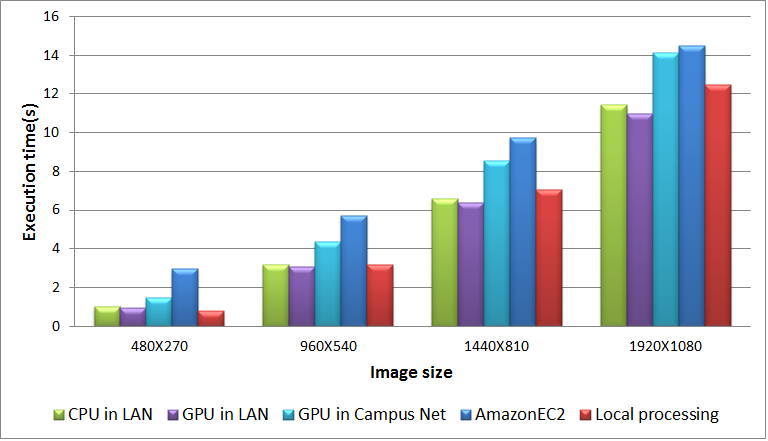
\includegraphics[height=4.5cm, width=7.3cm]{Figure/figure4-a}
}
\subfigure[Matrix Multiplication] {
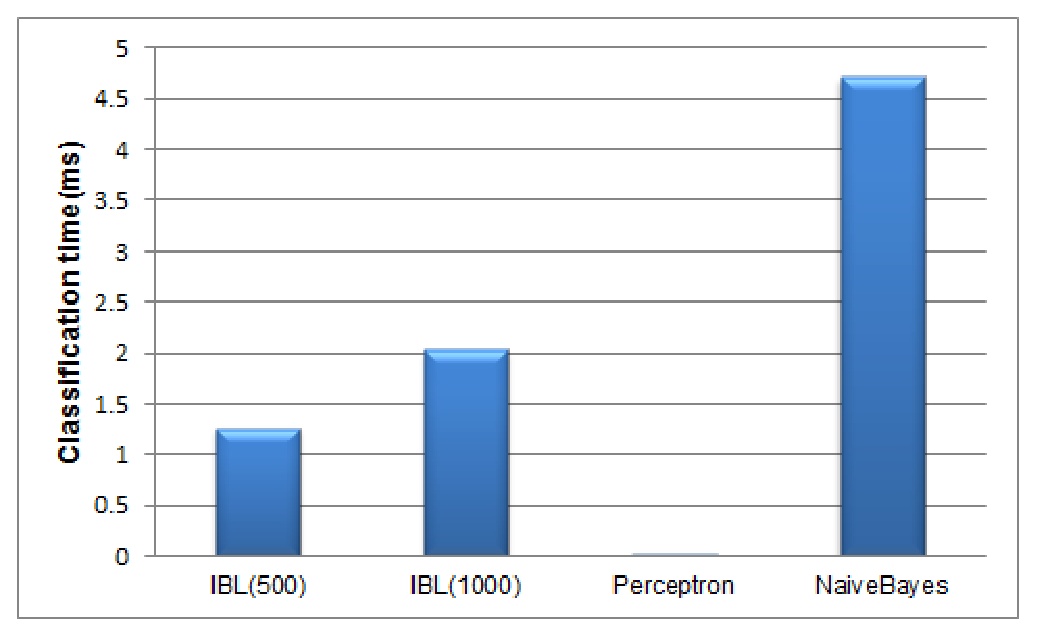
\includegraphics[height=4.5cm, width=7.3cm]{Figure/figure4-b}
}
\subfigure[Hidden Markov Model] {
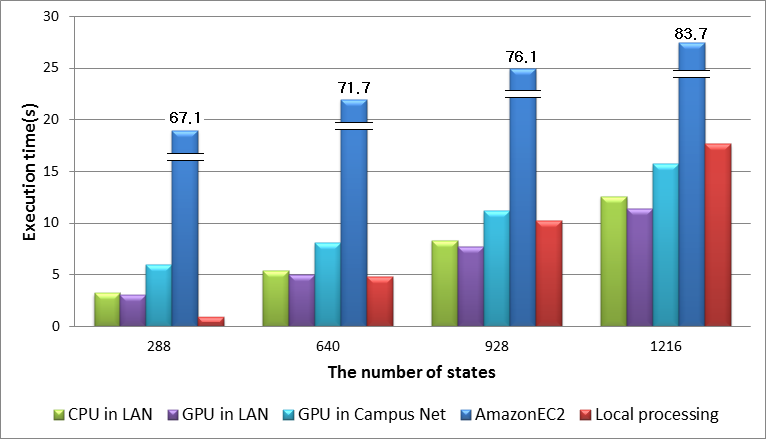
\includegraphics[height=4.5cm, width=7.3cm]{Figure/figure4-c}
}
\subfigure[N-body Physics] {
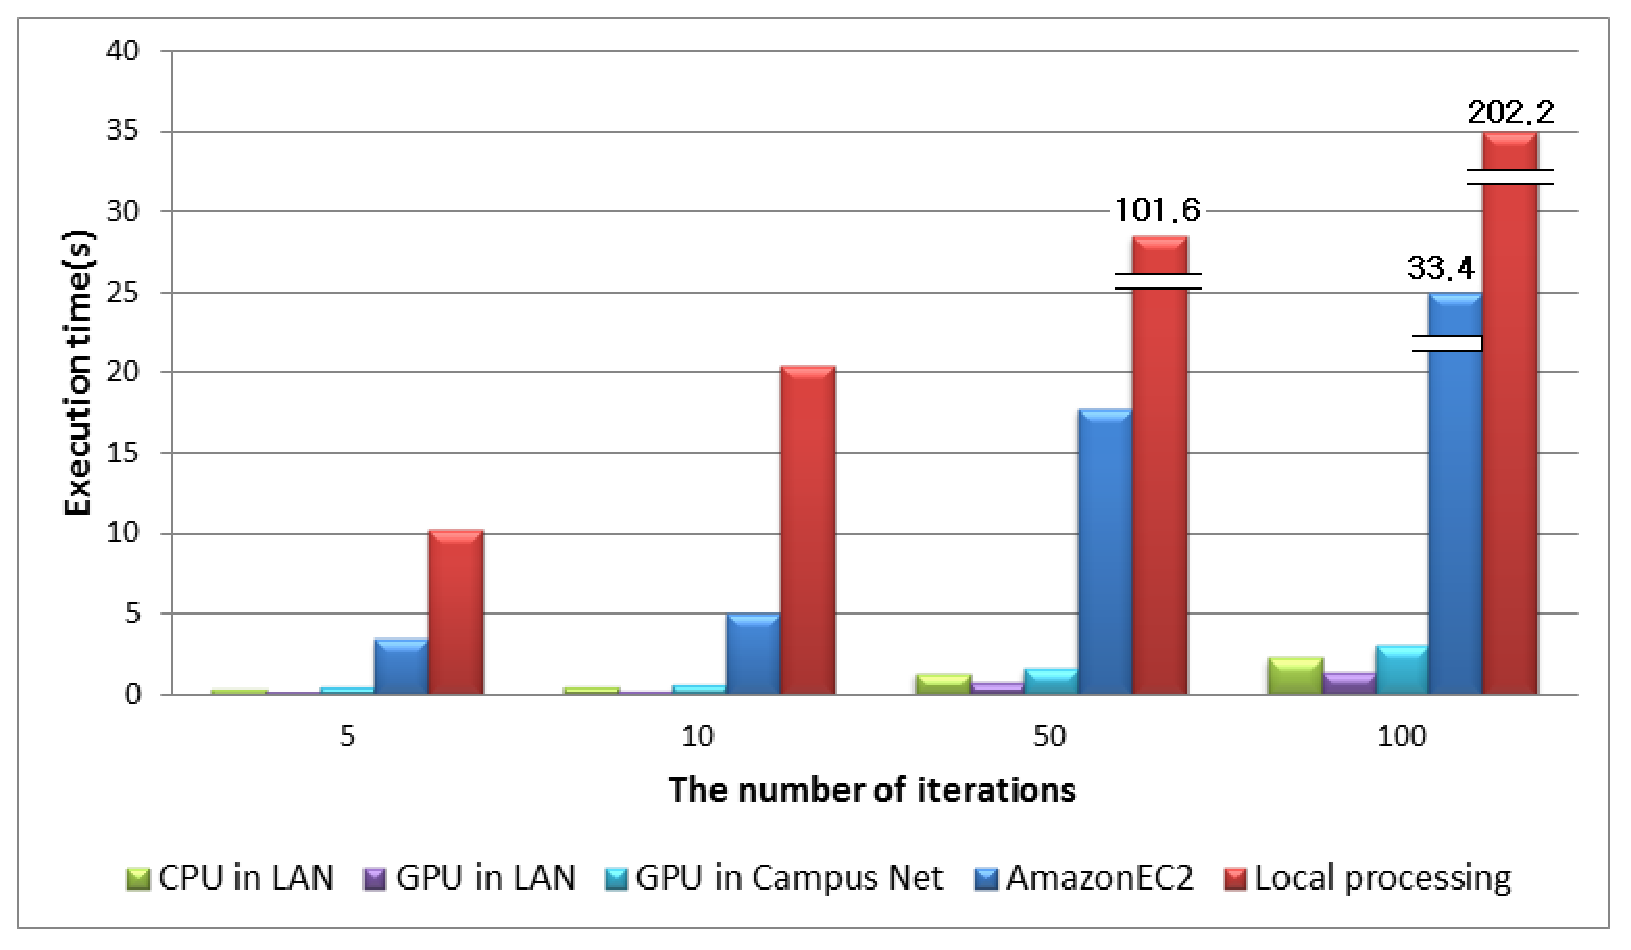
\includegraphics[height=4.5cm, width=7.3cm]{Figure/figure4-d}
}
\caption{
Execution time with various server setup}
\end{figure*}
%
\begin{figure*}[ht]
\centering
\subfigure[Sobelfilter] {
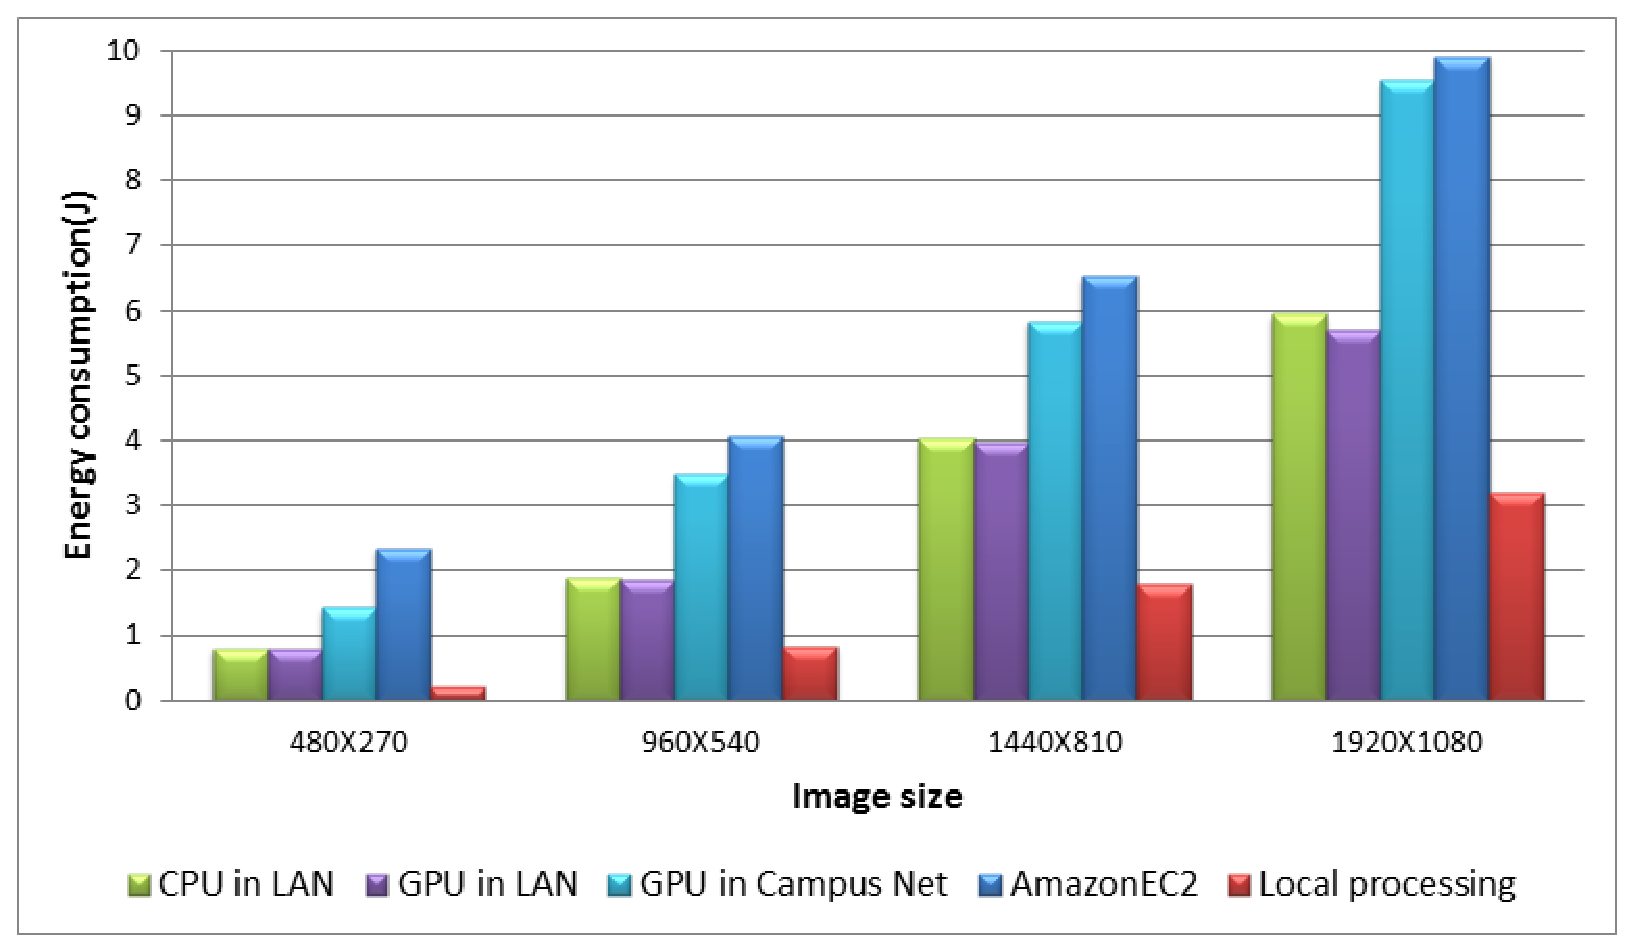
\includegraphics[height=4.5cm, width=7.3cm]{Figure/figure3-a}
}
\subfigure[Matrix Multiplication] {
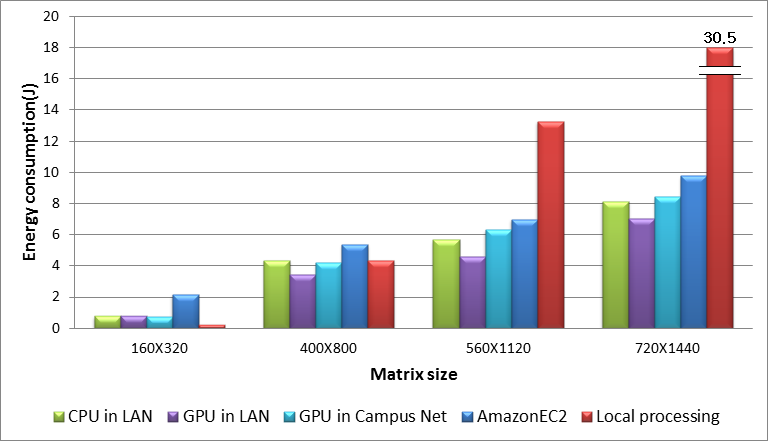
\includegraphics[height=4.5cm, width=7.3cm]{Figure/figure3-b}
}
\subfigure[Hidden Markov Model] {
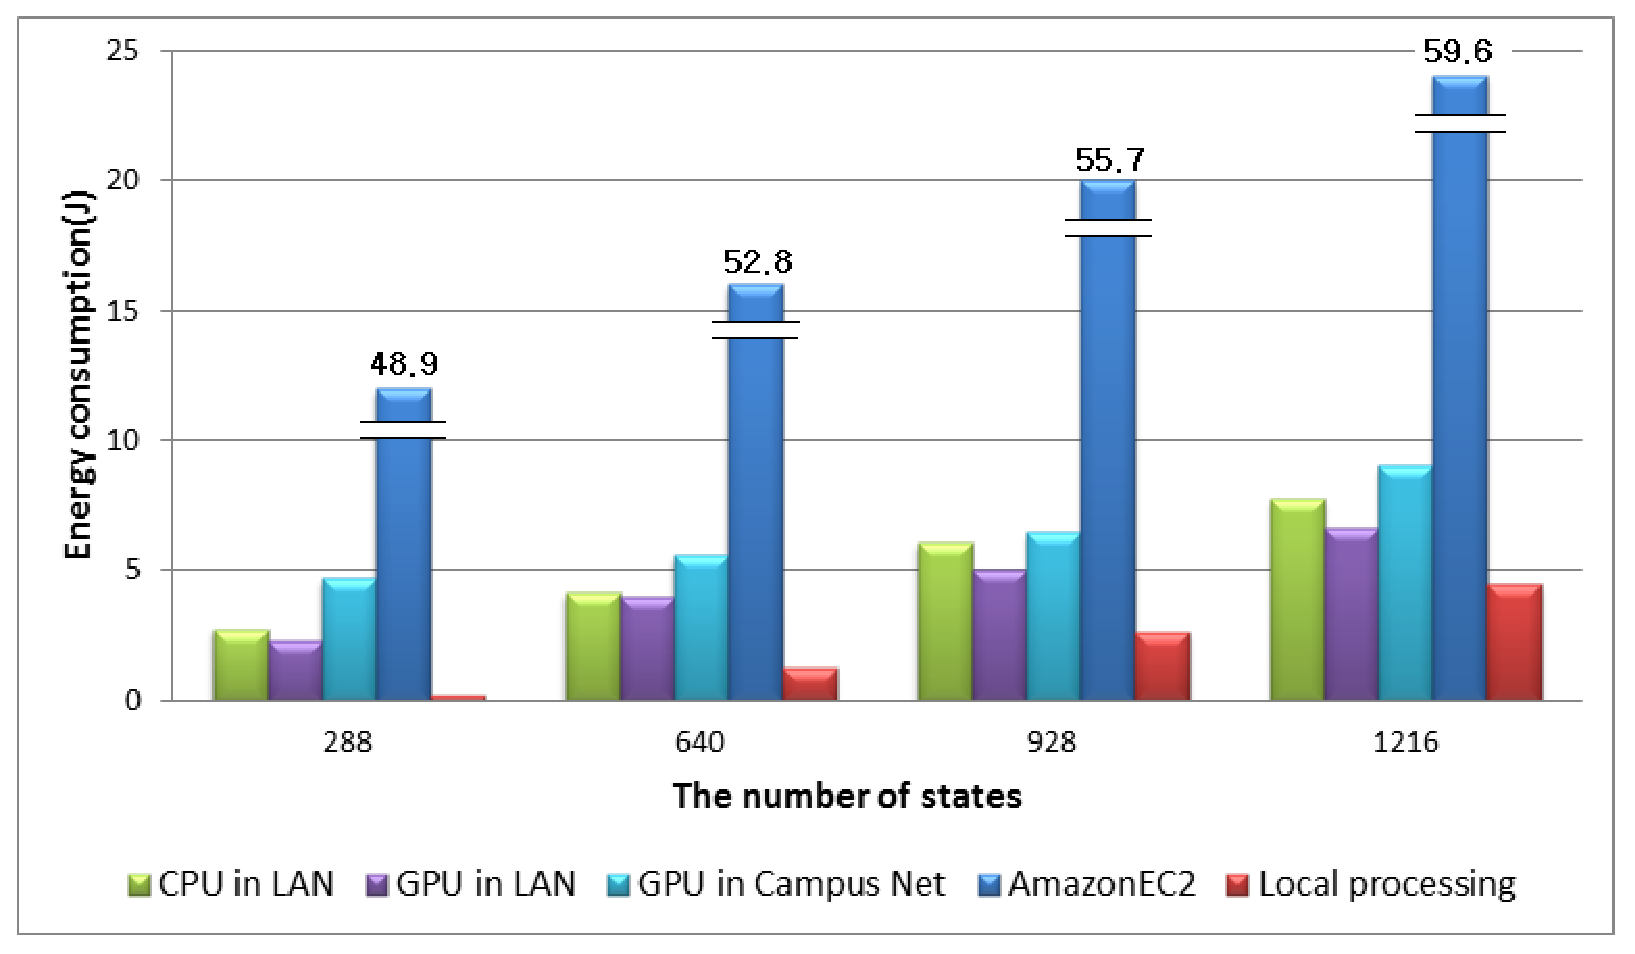
\includegraphics[height=4.5cm, width=7.3cm]{Figure/figure3-c}
}
\subfigure[N-body Physics] {
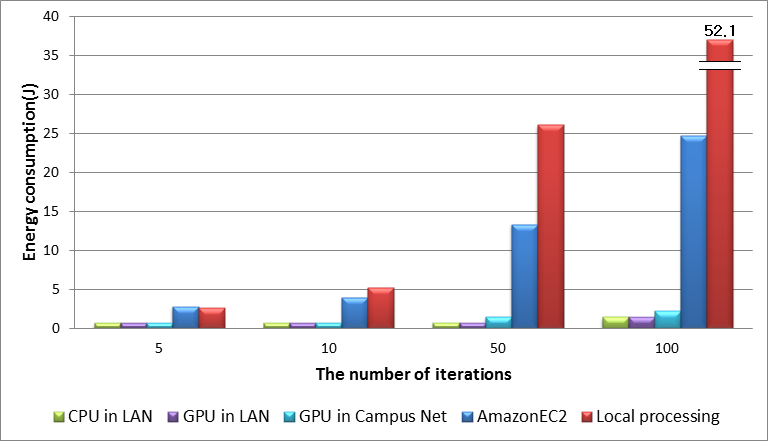
\includegraphics[height=4.5cm, width=7.3cm]{Figure/figure3-d}
}
\caption{
Energy consumption with various server setup}
\end{figure*}
%
\section{Related Works}
%
The research community has been investigating different methods to
offload computation for decades; however, remote execution to the cloud
has created new opportunities to explore novel offloading solutions.
%
In this section, we discuss the most recent proposals for mobile
computation offloading.\\
%which fall in the following categories:
%application partitioning, thread, application migration and distributed
%offloading framework.\\
%
\indent\textbf{Application Partitioning.} This approach involves selecting
portions of an application to execute remotely through the use of a
static or dynamic scheduler.
%
In Spectra~\cite{spectra}, developers identify functions in the
application that can be offloaded to a remote server over RPC.
%
By monitoring the CPU, file I/O, and bandwidth, Spectra 
decides at runtime which portions of the application should run locally
or remotely.
%
MAUI~\cite{maui} takes a similar approach but alleviates the process by
using many of the programming features in the .NET platform such as
method attributes, and the Reflection API.
%
Through the .NET Framework's virtual machine, MAUI is able to
dynamically serialize and ship \textit{remotable} methods and data to a
server proxy, thus leveraging the server's superior processing
capabilities while saving energy on the mobile device.
%
Cuckoo~\cite{cuckoo} takes a slightly modified approach by focusing more
on integrating with the Eclipse IDE; however, it requires developers to
implement both local and remote versions of their functionality, whereas
MAUI only requires annotations from developers.
%
Our approach may be classified as application partitioning similar to
Cuckoo because developers are required to re-implement portions of their
code for the OpenCL runtime environment; however, the developer does not
have to worry about the complications of shipping the workload to the
remote device.\\
%
\indent\textbf{Thread Migration.} The source code modification required for
most partitioning schemes can preclude adoption by many applications;
thread and process migration, on the other hand, can be achieved without
any source code modification.
%
CloneCloud~\cite{clonecloud} achieves this by employing thread migration
in the Dalvik Java Virtual Machine (JVM) by transferring all of the
thread state (thread stack, necessary heap objects and registers) to the
remote virtual machine.
%
When the remote thread completes, the results are merged back with the
local Dalvik JVM memory stack.
%
The authors of COMET~\cite{comet} developed a similar thread migration
technique by doing application VM synchronization through a distributed
shared memory (DSM) model.
%
Our proposed solution does not require any thread stack or heap
synchronization because the OpenCL framework requires explicit
declaration of input and output buffers for remote kernel execution.\\
%
\indent\textbf{Application Migration.} While the previous thread migration techniques
can be technically challenging to implement since they require memory
synchronization between the remote thread and other threads running
locally, Application migration does not have such requirements.
%
%All local threads have to block on "dirty" regions of the heap that has
%been offloaded to the remote server until the remote execution finishes
%and the memory is merged and released.
%
%Application migration does not have such requirements.
%
Hung et al.~\cite{hung} describes an application migration design that
leverages the \textit{onResume} and \textit{onPause} events of an
Android application as the markers for process migration.
%
The \textit{onPause} event occurs when a user switches to another
application.
%
The Android system requires that application states are stored on
persistent storage in case the operating system decides to shutdown in
the case of low memory situation.
%
Hence, Hung et al. creates a solution which uses the \textit{onPause}
event to force the application to save its state.
%
The state is then copied to a cloned VM running on the cloud and resumed
there until completion, then transferred back.
%
Our design automatically handles the state transfers between the local
and remote devices without relying on specific Android-based events.\\
%
\indent\textbf{Distributed Offloading Framework.} Various recent approaches
have focused on a totally different model requiring more effort from the
developers.
%
Proposals such as Mobile MapReduce (MMR)~\cite{mmr},
Sonora~\cite{sonora}, and Serendipity~\cite{serendipity} all expose a
distributed offloading framework for developers to adopt.
%
For example, MMR is a MapReduce system optimized for the constrained
networking conditions of mobile devices by taking into account bandwidth
and latency for efficient mobile device performance.
%
Sonora exposes a distributed stream-based programming model which
handles workload distribution and failures in a mobile network.
%
Serendipity provides an offloading framework for intermittently
connected mobile devices and does not rely on cloud services.
%
Our approach can also be classified as a distributed offloading
framework; however, instead of defining the system from scratch, we
reuse the workload offloading paradigms of the OpenCL
framework which provides more familiar and widely supported interfaces
for developers. 
%
\section{Conclusion}
%
In this paper, we proposed the OpenCL-based remote offloading framework
for mobile platforms through SocialVPN.
%
We implemented the prototype of our remote offloading framework on the
mobile platforms running Android OS and built the dynamic resource
discovery mechanism in which the mobile user is allowed to dynamically
and transparently discover the resources through IP multicasting on top
of SocialVPN.
%
Also, we characterized the benefits and the costs of our framework in
terms of total execution time and energy consumption through real
deployment of the prototype in local- and wide-area networks.
%
According to our evaluation, depending on the complexity of the workload
and the amount of data transfer, the proposed architecture can achieve more
energy efficient performance by offloading than executing locally.
%
In fact, in the case of matrix multiplication which is the
computation-intensive workload, offloading shows up to 9.2X speedup
depending on the matrix size, server's computing capabilities and network
conditions while it saves energy consumption up to 76.8\%.\\
%
\indent We currently seek to real mobile applications suitable to obtain the
benefits from our remote workload offloading framework such as face or
voice recognition.
%
With fault tolerant design, it is also possible that mobile devices
switch offloading to other available resources in the case of computing
node failure.
%
\section*{Acknowledgement}
This material is based upon work supported in part by the National Science
Foundation under Grant No. 0910812, 0758596, 0855031, and 1265341.
%
Any opinions, findings, and conclusions or recommendations expressed in
this material are those of the author(s) and do not necessarily reflect
the views of the National Science Foundation.
%
%\bibliographystyle{IEEEtran}
\bibliography{ipccc14}
\end{document}


